\documentclass{beamer}
\usepackage{amsfonts,amsmath,oldgerm}
\usetheme{sintef}
\usepackage{xeCJK}

\newcommand{\testcolor}[1]{\colorbox{#1}{\textcolor{#1}{test}}~\texttt{#1}}

%set CJK font
\setCJKmainfont{方正楷体简体.ttf}
\setCJKsansfont{方正楷体简体.ttf}
\setCJKmonofont{方正楷体简体.ttf}

\usefonttheme[onlymath]{serif}

\newcommand{\hrefcol}[2]{\textcolor{cyan}{\href{#1}{#2}}}

\title{The Use of Alignment-Free Analysis in Predicting the Evolution of Crucivirus}
% \course{Master's Degree in Computer Science}
\author{Yuxuan Liu}
% \IDnumber{1234567}
\date{July, 2023}
\begin{document}

\maketitle

\section{Introduction}

\begin{frame}{What is Virus?}
    \begin{itemize}
        \item Examples
    \end{itemize}
    \begin{columns}
        \begin{column}{0.5\textwidth}
            \centering
            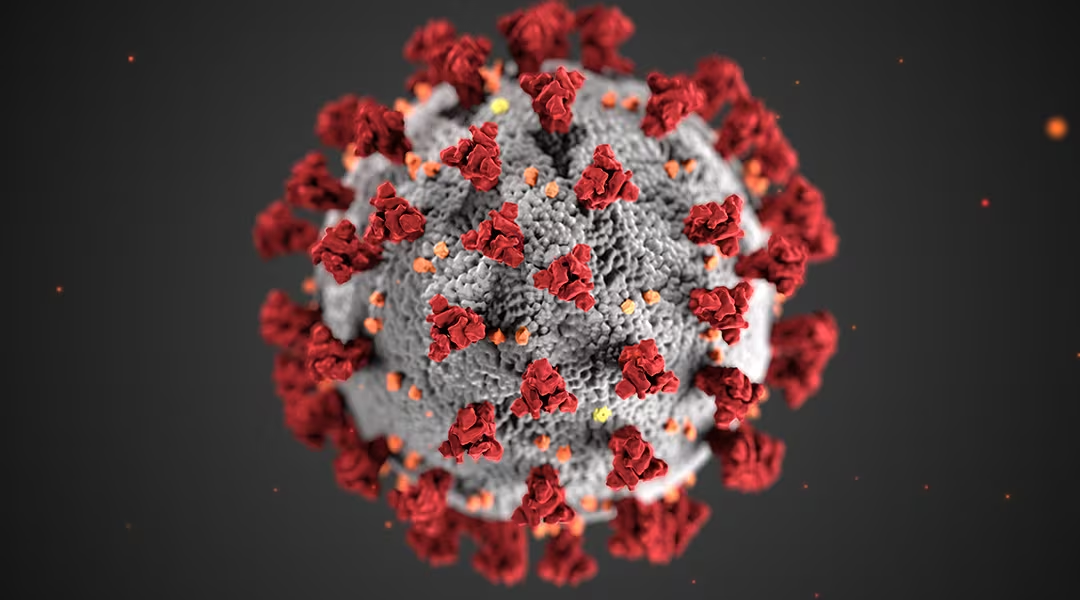
\includegraphics[scale = 0.18]{corona.png}
            
            Image by CDC
         \end{column}
         \begin{column}{0.5\textwidth}
         \centering
            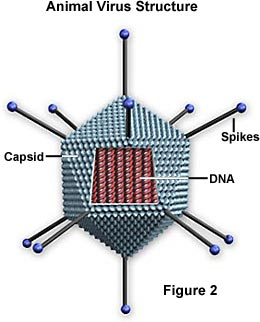
\includegraphics[scale = 0.5]{virusStructure.png}

            Image by Molecular Expressions
         \end{column}
    \end{columns}
\end{frame}

\begin{frame}{Effects of Virus}
    \centering
    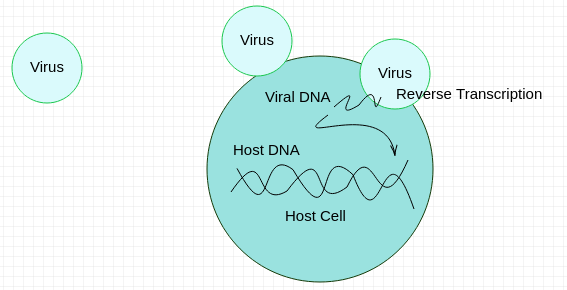
\includegraphics[scale = 0.5]{dnaMutation.png}
\end{frame}

\begin{frame}{DNA? RNA?}
    \centering
    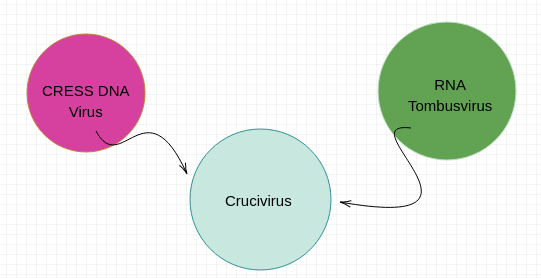
\includegraphics[scale = 0.5]{crucivirusStructure.png}
\end{frame}

\begin{frame}{Previous Research}
    \begin{columns}
        \begin{column}{0.5\textwidth}
            \centering
            Analyses researchers had used:
            \begin{itemize}
                \centering
                \item Phylogenetic analysis
                \item Network analysis
            \end{itemize}
        \end{column}
        \begin{column}{0.5\textwidth}
            \centering
            Analyses used in this project:
            \begin{itemize}
                \centering
                \item Alignment-Free Analyses
            \end{itemize}
        \end{column}
    \end{columns}
    
\end{frame}
\begin{frame}{Alignment-Free Analyses}
    \centering
    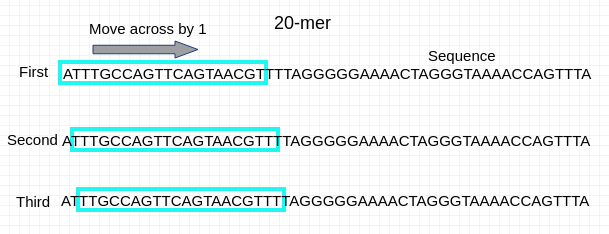
\includegraphics[scale = 0.7]{alignmentFree.png}
\end{frame}

\section{Methods and Materials}

\begin{frame}{Materials}
    \begin{columns}
        \begin{column}{0.5\textwidth}
            \centering
            
\includegraphics[scale = 0.11]{linux.png}
            
            Image by Coursera
         \end{column}
         \begin{column}{0.5\textwidth}
         \centering
            
\includegraphics[scale = 0.8]{numpy.png}

            Image by Numpy
         \end{column}
    \end{columns}
\end{frame}

\begin{frame}{Methods}
    \centering
    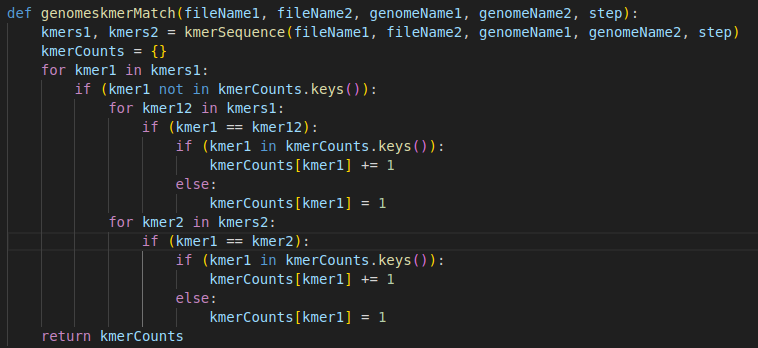
\includegraphics[scale = 0.5]{code.png}
\end{frame}

\section{Results}

\begin{frame}{Genome sense prediction}
\begin{center}
\begin{tabular}{||c c c c||}
    \hline
    Genome Name & CP Codon Bias & Rep Codon Bias & Genome Sense \\ [0.5ex]
    \hline\hline
    \texttt{Cruci\_CruV\_351} & T & A & ambisense \\
    \hline
    \texttt{Cruci\_CruV\_352} & T & A & ambisense \\
    \hline
    \texttt{Cruci\_CruV\_353} & T & A & ambisense \\
    \hline
    \texttt{Cruci\_CruV\_354} & T & T & unisense \\
    \hline
    \texttt{Cruci\_CruV\_355} & A & A & unisense \\
    \hline
    \texttt{Cruci\_CruV\_356} & C & C & unisense \\
    \hline
    \texttt{Cruci\_CruV\_357} & T & T & unisense \\
    \hline
    \texttt{Cruci\_CruV\_358} & T & A & ambisense \\
    \hline
    \texttt{Cruci\_CruV\_359} & T & A & ambisense \\ [1ex]
    \hline
\end{tabular}
\end{center}
\end{frame}

\begin{frame}{Pairwise Comparison}
    \centering
    Pairwise comparison of CP gene
    \begin{columns}
        \begin{column}{0.35\textwidth}
            \centering
            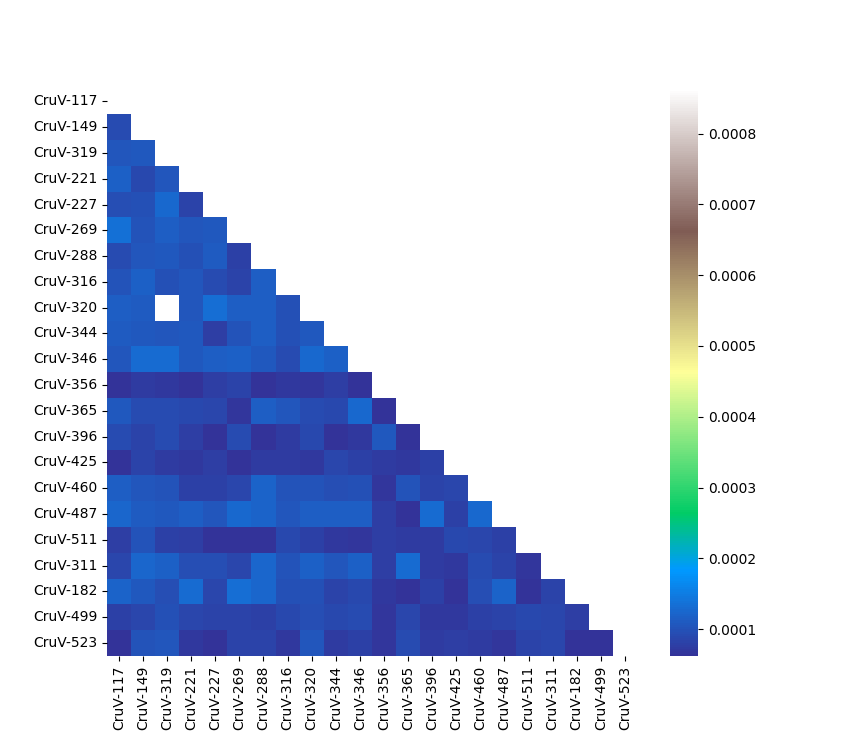
\includegraphics[scale = 0.25]{PairwiseCPHeatmap.png}
        \end{column}
        \begin{column}{0.65\textwidth}
            \centering
            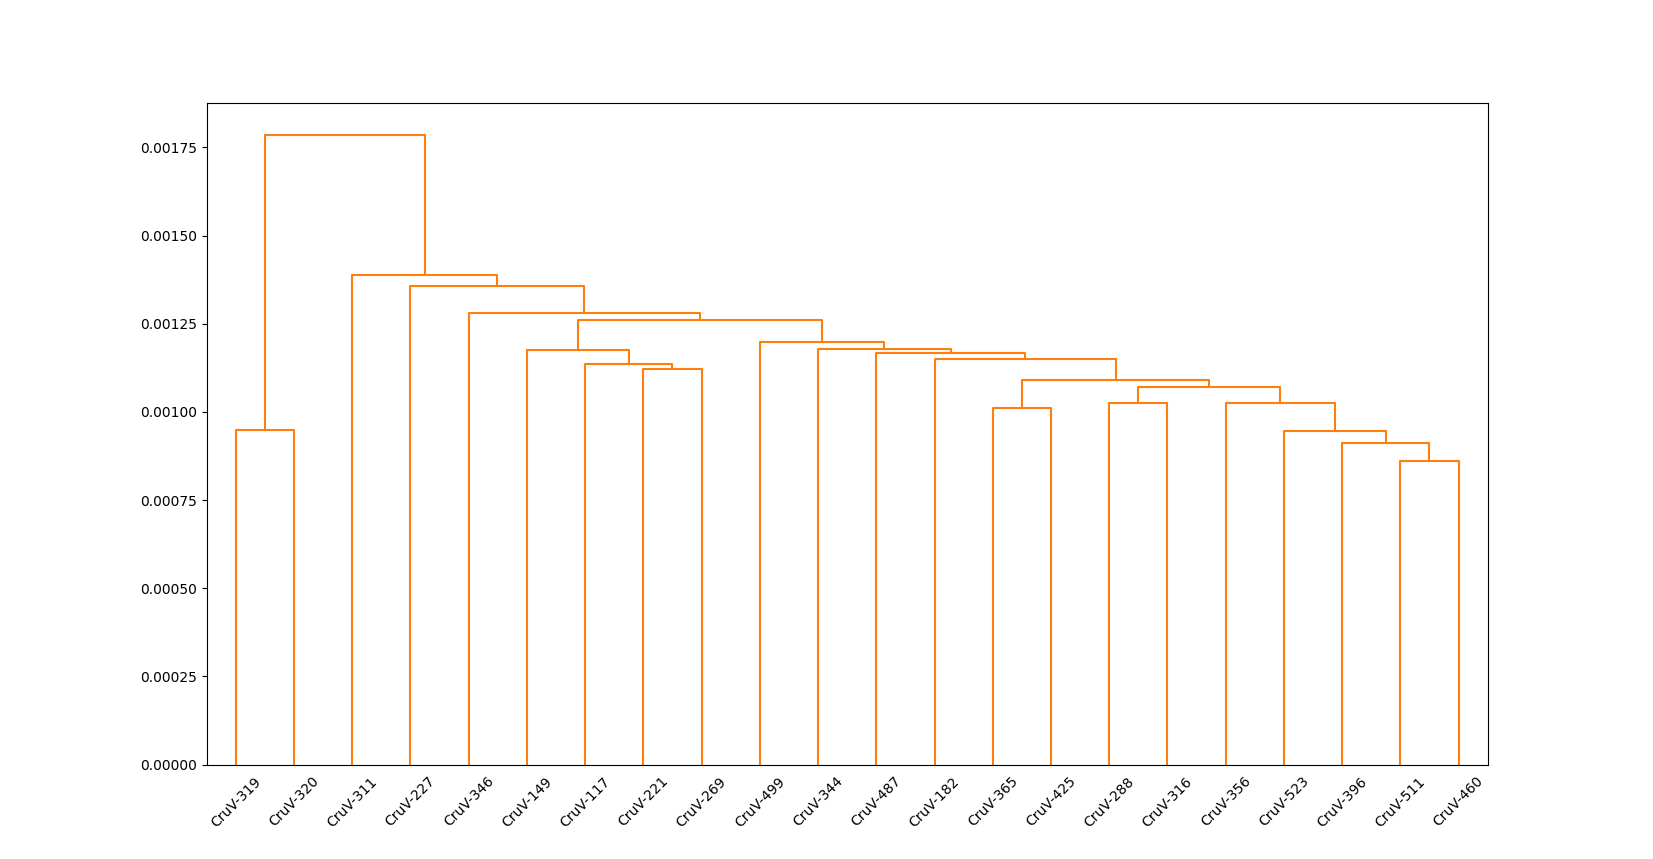
\includegraphics[scale = 0.25]{PairwiseCPDendrogram.png}
        \end{column}
    \end{columns}
\end{frame}

\begin{frame}{K-mer Similarity between CP and Rep Genes}
    \centering
    Distribution of K-mer Similarity between the CP and Rep genes of Crucivirus, RNA, and DNA Genomes
    
    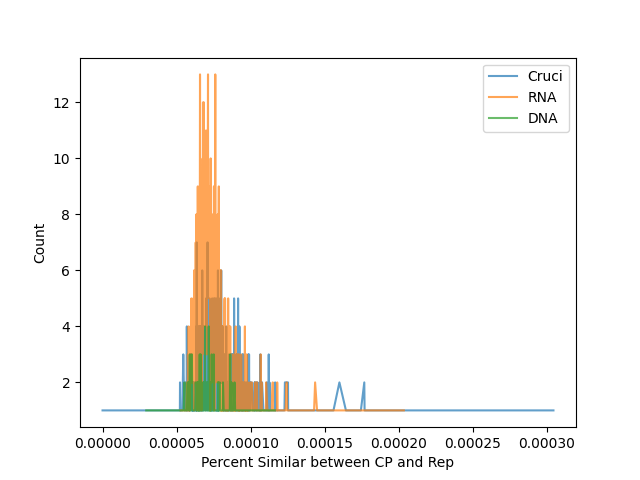
\includegraphics[scale = 0.5]{KmerSimilarityCpRep.png}
\end{frame}

\begin{frame}{Comparison of K-mers between Genomes}
    \centering
    Percentage of Similar K-mer between Crucivirus and DNA pairs

    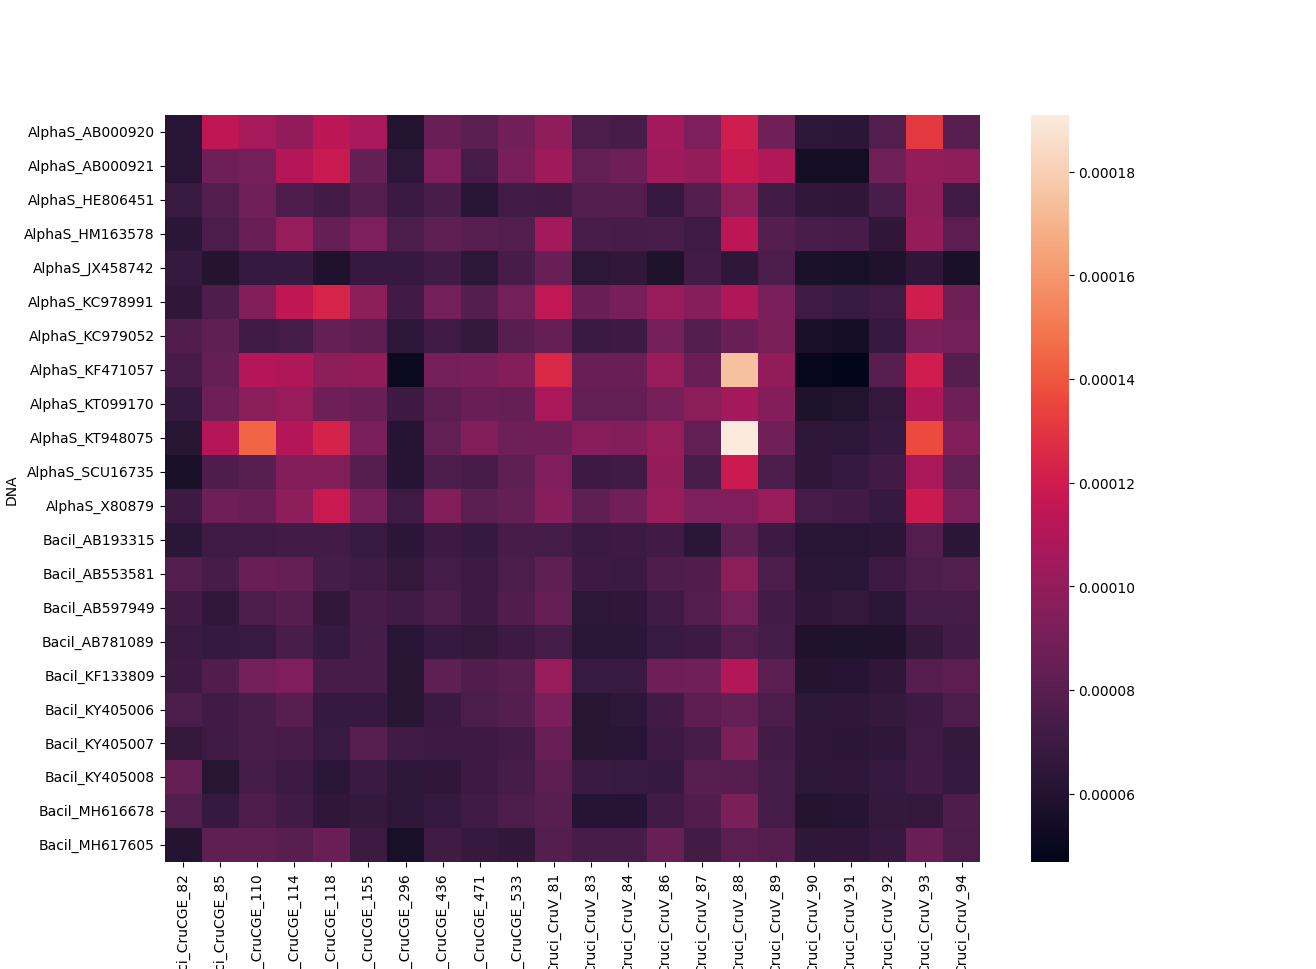
\includegraphics[scale = 0.25]{ComparisonBetweenDNAandCruci.png}
\end{frame}

\begin{frame}{Comparison of K-mers between Specific Genomes Examples}
    \centering
    Count of shared K-mers between Crucivirus-DNA pair
    \begin{columns}
        \begin{column}{0.5\textwidth}
            \centering
            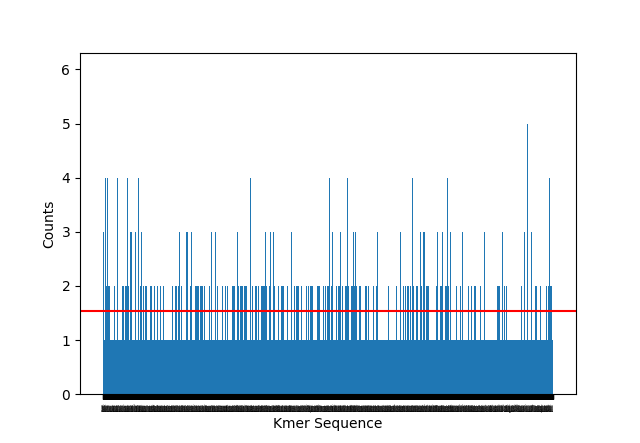
\includegraphics[scale = 0.5]{ComparisonBetweenCruci296DNAMH617605.png}
        \end{column}
        \begin{column}{0.5\textwidth}
            \centering
            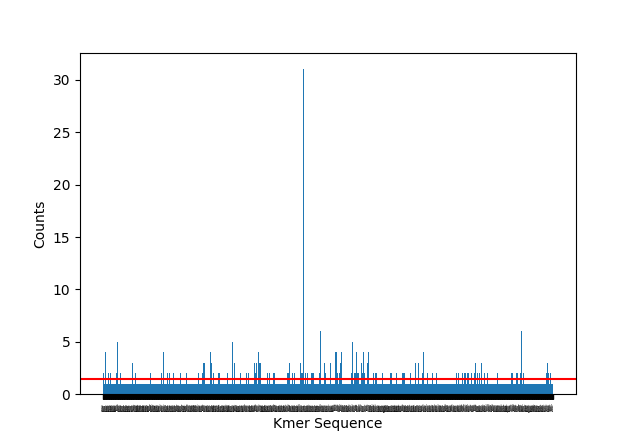
\includegraphics[scale = 0.5]{ComparisonBetweenCruci88DNAKT04807.png}
        \end{column}
    \end{columns}
\end{frame}

\backmatter
\end{document}
